\chapter{Machine learning based approach}


%====================================================================================================
\section{Concepts in machine learning}
Aim of this section is to define what exactly is understood by a term machine learning as well
as to introduce basic concepts that are common for all machine learning applications

%----------------------------------------------------------------------------------------------------
\subsection{Differences between knowledge and data based models}
While creating a model of physical processes one of two approaches may be used.
First, is the knowledge-driven model that as the name implies relays on knowledge of underlying
laws of physics that govern the process.
The main advantage of this approach is its high explainability and reliability as every parameter
of the model corresponds with some specific physical property.
However this model has a very significant downside, it requires detailed knowledge of physical
phenomena. This means that for complex processes it might be very difficult or even
impossible, at a~given moment, to create a model. Another drawback is that the complexity of
the process grows the computational cost of its model.
If those problem makes creating usable knowledge-based model impossible or economically
non efficient a data-driven approach may be used.
It model used is chosen arbitrarily with little or no relation to underlying physics,
then model parameters are adjusted until it will fit experimental data to the best of its
capability.
The main advantage of a data-driven approach is the lack of required knowledge on process 
inner workings, which allow prediction of events which exact mechanics have not 
yet been discovered.
Another element characteristic in the data-driven approach, that can be either advantageous or
disadvantageous, is the lack of direct correlation between the complexity 
of the process and computational cost of the model.
This is a very welcome trait for complex processes like orbital atomic clock ensembles.
The main disadvantage in comparison with the knowledge-driven approach is its lower reliability and
explainability. This is the main reason why the data-driven approach is usually avoided in
critical implementations. Another significant downside is a requirement of a large amount of
experimental data for model adjustment which means that in many cases this approach simply
cannot be used.
The last thing that must be said about the data-driven approach is that it still requires some
amount of knowledge to work efficiently as the selection of models that will be adjusted to
data requires some assumption. For example, the use of linear regression assumes that the model
is linear.

%----------------------------------------------------------------------------------------------------
\subsection{What is a machine learning algorithm}
Term machine learning describes subset of algorithms that adjusts parameter of other algorithms 
according to data. To provide more formal definition an algorithm can be described as a 
transformation function $\phi_{a}$ such that:
\begin{equation}
	\label{equ:algorithm_general}
	\mathcal{Y}_{a} = \phi_{a}(\mathcal{X},\Theta_{a}),
\end{equation}
where $\mathcal{Y}_{a}$ is set of algorithm responses, $\mathcal{X}$ is set of inputs 
and $\Theta_{a}$ is algorithm parameter set.
Input space $\mathcal{U}_{x}$ and response space $\mathcal{U}_{y}$ can be simply a numerical
space, in which case algorithm is called numerical algorithm, but can also represent more 
abstract concepts. For example in case of database software input space will consist of 
queries while response space will contain information stored in database as well as error 
status in case query was written incorrectly.
Machine learning algorithm, denoted as $\phi_{m}$ can also be described in that general form
however what is special in this case is that input space $\mathcal{U}_{m}$ consists of either :
\begin{equation}
	\label{equ:supervised_input}
	\mathcal{X}_{m} = \{\phi_{a}, \mathcal{X}_{a}, \mathcal{Y}_{a}, \Theta_{a} \},
\end{equation}
in case of supervised learning or just :
\begin{equation}
	\label{equ:supervised_input}
	\mathcal{X}_{m} = \{\phi_{a}, \mathcal{X}_{a}, \Theta_{a} \},
\end{equation}
in case of unsupervised learning.
In both cases response of machine learning algorithm is described as a:
\begin{equation}
	\label{equ:ml_response}
	\mathcal{Y}_{m} = \{\hat{\Theta}_{a}, E_{a}\},
\end{equation}
where $\hat{\Theta}_{a}$ is adjusted set of parameters and $E_{a}$ is value prediction 
error for this new set of parameters.
Aim of machine learning algorithm is to adjust parameters $\Theta_{a}$ of given algorithm 
$\phi_{a}$ in such a way to minimize error $E_{a}$ for given data. In case of supervised learning
a correct response $\mathcal{Y}_{a}$ for inputs is known where in case of unsupervised learning
only input set $\mathcal{X}_{a}$ is known. In order to avoid confusion parameters of machine 
learning algorithm $\Theta_{m}$ will be referred to as a \textit{metaparameters}. 
Exact set of meteaparameters vary between specific algorithms, however there is one 
crucial metaparameter that will appear in every machine learning algorithm.
That metaparameter is error function as it is required for error value calculation and as 
minimization of that value is goal of machine learning it is mandatory to be able to calculate it.

%----------------------------------------------------------------------------------------------------
\subsection{Error function}
As an error function is used for calculation of value that will be minimized by a machine 
learning algorithm correct choice of that function is crucial decision when designing such
algorithm.
Due to scope of this work attention will be given only to error function used in supervised 
learning of numerical algorithms.
Error for single pair of predicted value $\hat{y}$ and actual value $y$ can be described as
distance between them in response space $\mathcal{U}_{y}$:
\begin{equation}
	\label{equ:dist_general}
	E = f_{DIST}(\hat{y},y),
\end{equation}
where $f_{DIST}$ is distance function, alternatively called metric.
Distance function is a function that gives a distance between each pair of point elements of a set.
If a set have a distance function defined it is called a metric space. 
In order to be classified as a metric function $f_{DIST}$ over a Cartesian square of a universe 
$\mathcal{U}$ it must display following properties:
\begin{enumerate}
	\item $f_{DIST} : \mathcal{U} \times \mathcal{U} \to \mathbb{R}^{+}$
	\item identity of indiscernibles : $f_{DIST}(x_{0}, x_{1})=0 \leftrightarrow x_{0} = x_{1}$,
	\item symmetry : $f_{DIST}(x_{0},x_{1})=f_{DIST}(x_{1},x_{0})$,
	\item triangle inequality : $f_{DIST}(x_{0},x_{1}) \leq f_{DIST}(x_{0},x_{2}) +
		f_{DIST}(x_{1},x_{2})$. 
\end{enumerate}

There are many types of metrics however within scope of this work attention will be given only to
distance functions related to $\ell$ norms.
As such error function for single prediction will be described as: 
\begin{equation}
	\label{equ:dist_norm}
	E = \Vert (\hat{y}-y) \Vert_{k},
\end{equation}
where notation $\Vert \bullet \Vert_{k}$ describes $k$ norm of given value.
Norm is a function from a real or complex vector space to the non negative real number space
that describes distance of a point from the origin.
Origin is the point for which values of all dimension are equal to zero, in case of calculating
$\ell$ norm for difference between two points subtrahend is treated as a origin point.
General equation describing a $\ell_{k}$ norm in $n$ dimensional space is:
\begin{equation}
	\label{equ:ell_norm}
	\Vert x \Vert_{k} = (\vert x_{0} \vert^{k} + \vert x_{1} \vert^{k} + \cdots +
	\vert x_{n} \vert^{k})^{1/k},
\end{equation}
where $\vert x \vert$ is an absolute value of $x$.
\begin{figure}[htb] 
	\label{fig:l_norms}
	\centering
	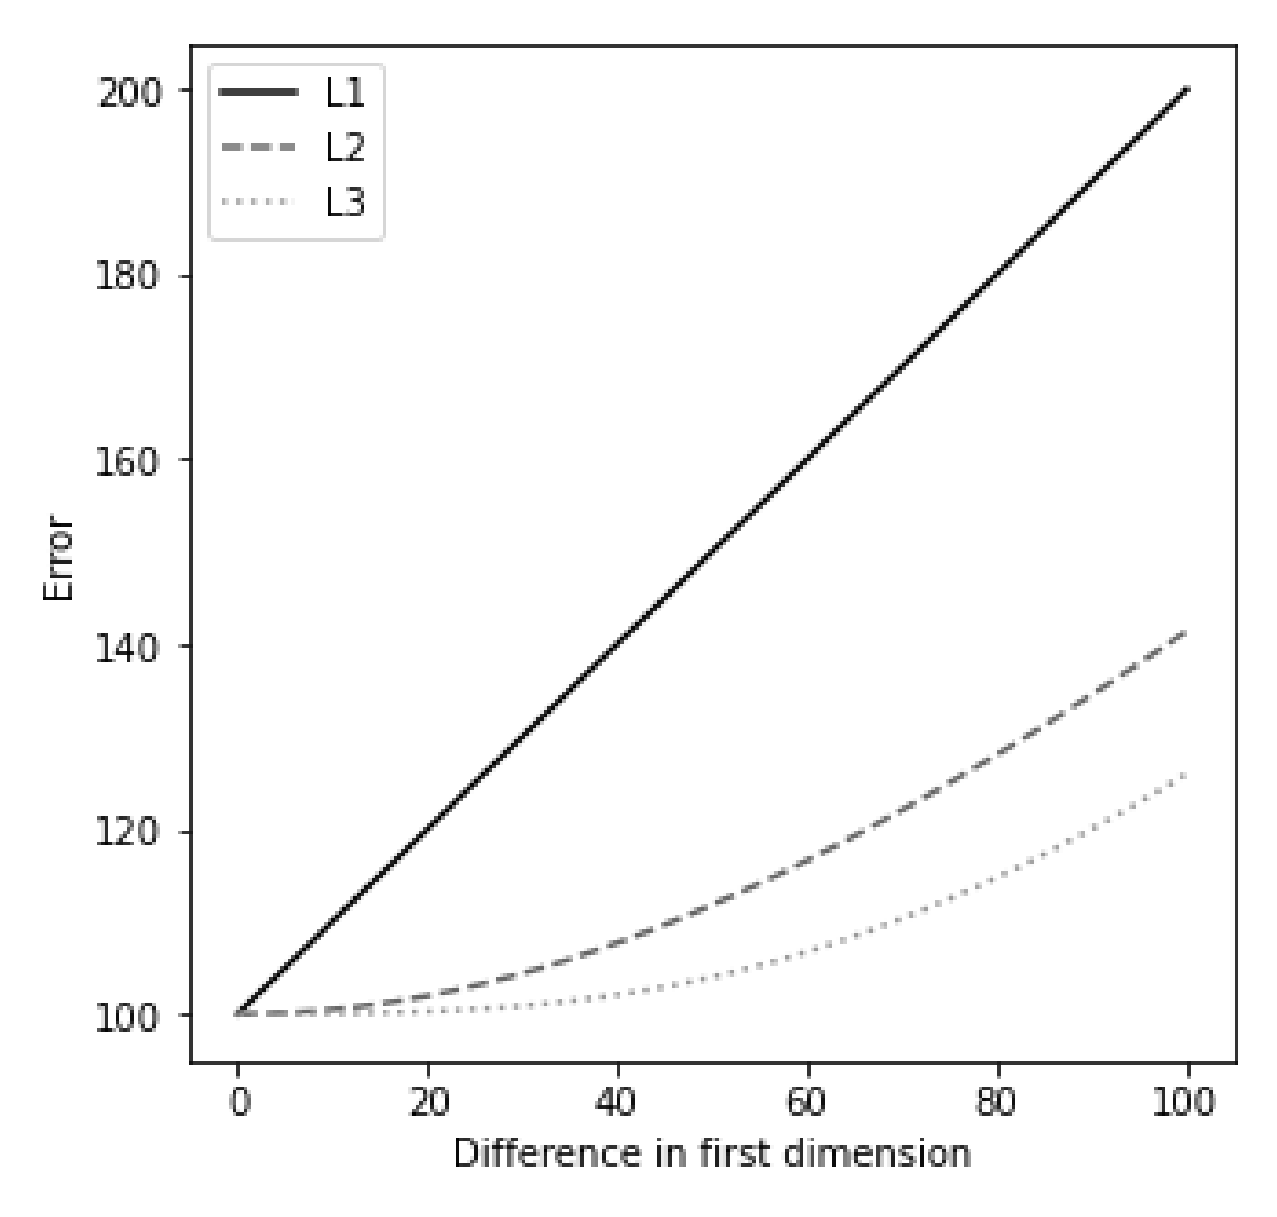
\includegraphics[width=0.5\textwidth]{figures/l_norms}
	\caption{Relation between error and difference in first dimension values with second 
	dimension difference at constant 100}
\end{figure}
\textbf{TODO: DESCRIBE WHY USE GIVEN NORMS IN MORE DETAIL}
Norms usually used in error calculation are $\ell_{1}$ and $\ell_{2}$, due to their frequent use
not only in this field they are given specific names.
Norm $\ell_{2}$ is called Euclidean norm and is equivalent to intuitive understanding of distance
while norm $\ell_{1}$ is called Manhattan distance and is related to distance between points on 
grid.
Euclidean distance is used for calculation of Root Mean Squared Error (RMSE). If we define 
knowledge base $K$ as a set of pairs $(x,y)$ where $x$ is input and $y$ an expected output
while prediction is realised by hypothesis $\hat{y} = h(x,\phi)$ error can be described as:
\begin{equation}
	\label{equ:mse}
	f_{RMSE}(K,h) = \sqrt{\frac{1}{\vert K \vert} \sum_{(x,y) \in K}(h(x,\phi)-y)^2},
\end{equation}
where $\vert K \vert$ is cardinality of knowledge base.
Manhattan distance is in turn used to calculate Mean Average Error (MAE):
\begin{equation}
	\label{equ:mae}
	f_{MAE}(K,h) = \frac{1}{\vert K \vert} \sum_{(x,y) \in K}\vert (h(x,\phi)-y)\vert.
\end{equation}
Those two error values will be used in this work.


%----------------------------------------------------------------------------------------------------
\subsection{Deep learning}
At time when experiments described in this dissertation were conducted a new approach to 
machine learning called Deep Learning (DL) became highly popular.
Due to that popularity term deep learning is often overused and misrepresented marketing 
purposes. In this section an attempt will be made to explain what exactly constitutes as a
deep learning and describe what sort of challenges.
Term deep learning can be applied only to a subset of machine learning algorithms that have
layer based architecture, usually a neural networks.
In such implementation whole data processing algorithm can be described as a transformation:
\begin{equation}
	\label{equ:spaces1}
	\phi = \mathcal{U}_{OBS} \Rightarrow \mathcal{U}_{RES},
\end{equation}
where $\mathcal{U}_{OBS}$ is called observation space and $\mathcal{U}_{RES}$ is response space.
In case of simple single layer system observation space is directly transformed into a 
response space, however in case of multi layer model there are intermediate encoding spaces.
In such case representation spaces are numbered by index of layer which outputs them. 
So in case of $n$ layer system it would be $\{\mathcal{U}_{0}, \mathcal{U}_{1},
\cdots, \mathcal{U}_{n}\}$ where indexes $0$ and $n$ are special as 
$\mathcal{U}_{0}=\mathcal{U}_{OBS}$ and $\mathcal{U}_{n}=\mathcal{U}_{RES}$.
In that case a function transforming observation into a reaction can be described as a 
convolution of multiple encoding function.
\begin{equation}
	\label{equ:spaces_transform}
	\phi = \phi_{1} \otimes \phi_{2} \otimes \cdots \otimes \phi_{n}.
\end{equation}
Transformation $\phi_{n}$ is called output layer, while other transformation are referred to
as a hidden layers as their result is not visible during normal operation of algorithm.
Until recently almost all architectures used a single hidden layer and architectures with more
than 3 hidden layers were almost unheard of.
This is due to three issue that show up in systems with higher amount of layer: signal vanishing,
signal explosion and rise in computation due to high parameter count.


%====================================================================================================
\section{Regression approximation}

%----------------------------------------------------------------------------------------------------
\subsection{Linear regression}
Linear predictor function is a linear combination of a set of coefficients and explanatory 
variables (independent variables), whose value is used to predict the outcome of a
dependent variable. Linear predictor is described as:
\begin{equation}
	\label{equ:linear_predictior}
	\hat{y} = \Theta_{0} + \Theta_{1}x_{1} + \cdots + \Theta_{n}x_{n},
\end{equation}
where $\hat{y}$ is predicted value,$n$ is feature count, $x_{i}$ is value of i-th feature
and $\Theta_{j}$ is j-th parameter.
Parameter $\Theta_{0}$ is special as it is not corresponding to any feature, that parameter
is called a \textit{bias term} or just \textit{bias}.
Predictor will return value of bias if all inputs are set to zero.
Function that allows prediction is called hypotesis function and is written as $\hat{y} = h(x)$.
With assumption that input vector for such function is $x=[1, x_{1}, \cdots, x_{n}]$ then 
a hypotesis function of a linear predictor can be defined as:
\begin{equation}
	\label{equ:linear_hyp}
	\hat{y} = h_{\Theta}(x) = \Theta^{T}\cdot x.
\end{equation}
To define how well prediction fit actuall data a error function must be selected and then one
of to approaches for minimizing it must be applied. Gradient based approach will be described 
is section \ref{sec:gradient} here a analytical approach based on a normal equation will be shown.
To derieve normal equation a MSE will be used as a error function, if other function would be 
selected a different normal equation would be a result.
In matrix notation hypothesis function can be described as :
\begin{equation}
	\label{equ:linear_hyp_matirx}
	\hat{Y} = h_{\Theta}(X) = \Theta^{T}\cdot X,
\end{equation}
where $X$ is input matrix such that each row represent single feature and each column 
single observation:
\begin{equation}
	\label{equ:input_matrix}
	X_{n\times m}=\left( \begin{array}{c c c c c}
		1&1&1&\cdots&1\\
		x^{(1)}_{1}& x^{(2)}_{1}& x^{(3)}_{1}& \cdots& x^{(m)}_{1}\\
		x^{(1)}_{2}& x^{(2)}_{2}& x^{(3)}_{2}& \cdots& x^{(m)}_{2}\\
		\vdots&\vdots&\vdots&\ddots&\vdots\\
		x^{(1)}_{n}& x^{(2)}_{n}& x^{(3)}_{n}& \cdots& x^{(m)}_{n}\\
	\end{array}\right),
\end{equation}
where $x^{(i)}_{j}$ denotes value of $j$ feature of $i$ observation.
%----------------------------------------------------------------------------------------------------
\subsection{Polynomial regression}

%----------------------------------------------------------------------------------------------------
\subsection{Support vector machine}


%====================================================================================================
\section{Gradient based optimization}
\label{sec:gradient}

%====================================================================================================
\section{Neural networks}

%----------------------------------------------------------------------------------------------------
\subsection{Feed forward neural networks}

%----------------------------------------------------------------------------------------------------
\subsection{Simple recurrent neural networks}

%----------------------------------------------------------------------------------------------------
\subsection{Networks with long term memory}

